% ----------------------------------------------------------------
% achemso --- Support for submissions to American Chemical
%  Society journals
% Maintained by Joseph Wright
% E-mail: joseph.wright@morningstar2.co.uk
% Originally developed by Mats Dahlgren
%  (c) 1996-98 by Mats Dahlgren
%  (c) 2007-2008 Joseph Wright
% Released under the LaTeX Project Public license v1.3c or later
% See http://www.latex-project.org/lppl.txt
% 
% Part of this bundle is derived from cite.sty, to which the
% following license applies:
%   Copyright (C) 1989-2003 by Donald Arseneau
%   These macros may be freely transmitted, reproduced, or
%   modified provided that this notice is left intact.
% ----------------------------------------------------------------
% 
% The achemso bundle provides a LaTeX class file and BibTeX style
% file in accordance with the requirements of the American
% Chemical Society.  The files can be used for any documents, but
% have been carefully designed and tested to be suitable for
% submission to ACS journals.
% 
% The bundle also includes the natmove package.  This package is
% loaded by achemso, and provides automatic moving of superscript
% citations after punctuation.

\documentclass[
%journal=ancac3, % for ACS Nano
%journal=acbcct, % for ACS Chem. Biol.
%journal=jacsat, % for undefined journal
manuscript=article]{achemso}

\usepackage[version=3]{mhchem} % Formula subscripts using \ce{}
\usepackage{graphicx}
\newcommand*{\mycommand}[1]{\texttt{\emph{#1}}}

\author{Ananthan, M.}
\email{ananthan@mecheng.iisc.ernet.in}
\affiliation{Department of Mechanical Engineering, Indian Institute of Science, Bangalore}

\title[\texttt{achemso} demonstration]
{Multiscale Simulation of Thin Films in Multiphase~flows}

\begin{document}

\begin{abstract}
A common scenario in multi-phase flow simulation  is the formation of thin fluid films in between colliding fluid masses or between a fluid mass and a surface.These films are very thin ( O(100nm) ) and during the DNS of multi-phase flows it is impractical to resolve their thickness fully due to various reasons outlined below.Our approach here is to couple a complex thin film model found analytically to a standard interface capturing technique like Volume of Fluid method so that we can capture the formation and evolution of thin films which comes into existence in the sub-grid thickness.
\end{abstract}


\section{Introduction}

Even though numerical simulation of multiphase-flows is a fast growing field ,Direct Numerical Simulation
(DNS) of a real two fluid system is very challenging with our current capabilities even when these systems are completely described by continuum theories.The main challenge is the existence of different scales in the flow which can vary over two order of magnitude.The need for multiscale approach is evident since most multiphase-flows of interest involve a large number of bubbles and drops with their length scales many times that of the dominant flow length scale.

The classical example~\cite{1} is we assume that we need O(10) grid points to resolve a drop that is 0.5 mm in diameter then then we need O(billion) grid points to resolve a chamber that is 10 cm cubed.
Most industrial systems are larger and most bubbles and drops are much smaller.E and Engquist ~\cite{2} in their review paper have classified multiscale problems in multiphase-flows in to two categories:

\begin{figure}[h]
 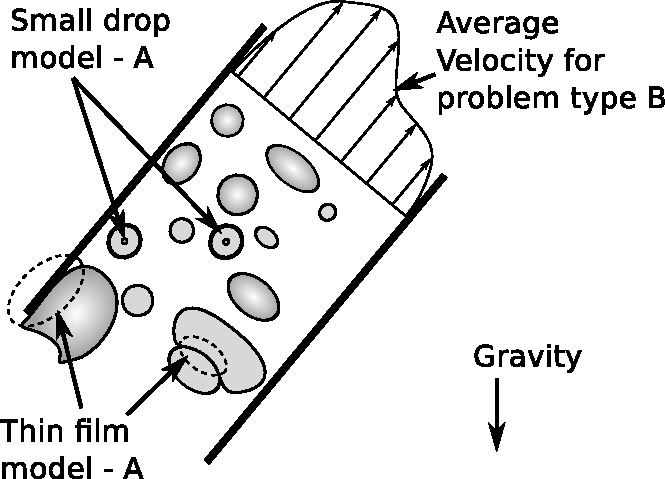
\includegraphics[scale=0.7]{drawing}
 \caption{Bubbly Flow in an inclined channel}
  \label{sch:example}
\end{figure}

Type A problems: Dealing with Isolated problems.

Type B problems: Constitutive modeling based on Microscopic models.

Tryggvason has provided a graphical representation of these two categories of problems.

The fig.1 shows both categories of problems for a bubbly flow in an inclined channel.Problem B is the classical averaging method in multiphase flow modelling, which results in a model which captures the aspects of the flow relevant to us without resolving the flow fully.Problem A is how we deal with unresolved thin films,threads and droplets that appear as flow progresses.

We are interested in type A problems especially those involving thin liquid films, which are formed when two fluid masses collide or when a fluid drop hits a surface.As we have already discussed , the length scales involved in these film drainage process vary in a wide range of length scale from external flow which exceeds droplet diameter to nanometer scales where van der Waals force becomes active.It is computationally impractical to capture this in a fixed grid method.Theoretically the features of thin films can be captured by local Adaptive Mesh Refinement(AMR) but it is not recommended because of the following reasons:

1.AMR increases the complexity of the computation and results in increased computational time.

2.AMR has to be done in stages i.e. the adjacent grid sizes should only differ by about a factor of two, so the refinement might end up using all the available grid resolution.

3.Some forces like van der Waals forces will only "act up" in a very small length scale and incorporating them in the conventional Navier-Stokes equation is computationally difficult.

So in any grid based method the final stages of film drainage will always be at sub-grid scale, and in conventional interface capturing methods two approaching interfaces will automatically coalesce when the two interfaces are close to each other and that distance is in the order of grid dimension.~\cite{3}.This is called as numerical coalescence and it is unphysical in nature.

In this study we are using an interface capturing technique like Volume of Fluid to capture the interface up to the sub-grid level then we couple it with an  analytically derived thin film model to capture the evolution of the thin film and drainage in the final stages.Thomas etal ~\cite{4} used this method for a front tracking/finite volume code where he used a simple thin film equation ignoring the effects of surface tension and van der Waals forces.The results capture the evolution of films thinner than the grid spacing reasonably well.Kwakkel etal ~\cite{5} has used a this method for a droplet laden flow.In their work they have coupled Coupled Level Set Volume of Fluid method~\cite{6} with a droplet coalescence model of Zhang and Law ~\cite{7}. In the CLSVOF method each droplet has its own locally defined marker functions. This prevents the problem of numerical coalescence in conventional Level-Set and Volume-of-Fluid methods when two droplet interfaces are less than one grid cell apart from each other. In their present model coalescence is based on a computationally efficient film drainage model, which predicts if and when two colliding droplets will coalesce. If the contact time between two colliding droplets exceeds the predicted film drainage time, coalescence is numerically accomplished by merging the marker functions of the two separate droplets.
The Thin Film model we are using ~\cite{8} is modeled from Navier-Stokes equation where surface tension forces and intermolecular forces are significant.Detailed derivation of the thin film equation can be seen in Williams and Davis~\cite{9}.

\subsection{Thin Film Equation}

Consider Continuity and Navier-Stokes equation for a thin film
\begin{equation}
\nabla \cdot \vec{V} = 0
\end{equation}
\begin{equation}
\rho \frac{D\vec{V}}{Dt} = \rho \left[ \frac{\partial{\vec{V}}}{\partial{t}} + \Big( \vec{V} \cdot \nabla \Big) \vec{V} \right] = -\nabla P + \nabla \Pi + \mu \nabla^{2} \vec{V}
\end{equation}
Doing Order of magnitude analysis we get
\begin{equation}
\frac{\partial{\Big( P - \Pi \Big)}}{\partial{x}} = \mu \frac{\partial^2{u}}{\partial^2{y}}
\end{equation}
\begin{equation}
\frac{\partial{\Big( P - \Pi \Big)}}{\partial{y}} = 0
\end{equation}

This  is the Thin Film Approximation where $ \Pi $    is the Disjoining pressure of the film due to excess intermolecular interactions.

Consider a thin film on a flat solid surface with another fluid on top of the film.We use the boundary conditions of no slip on the surface.Also we assume there is no shear force on the top surface i.e, free 
surface.

\begin{center}
  \begin{figure}[h]
 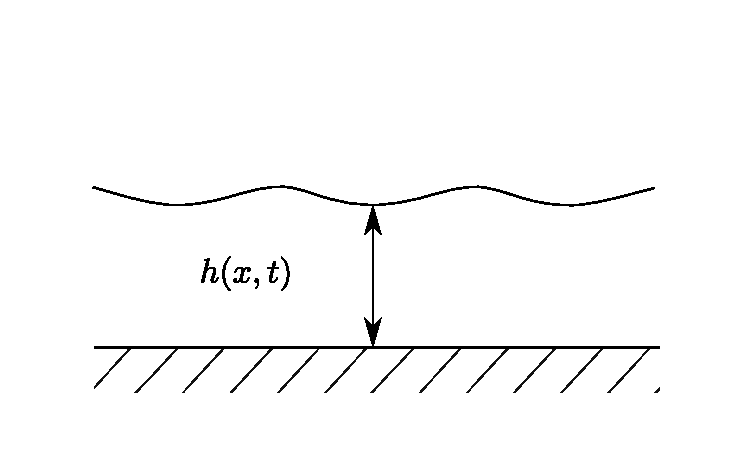
\includegraphics[]{Bubble_impinge.pdf}
 \caption{Thin fluid film on a substrate} \label{fig:impinge}
\end{figure}
\end{center}

\begin{equation}
\frac{\partial{u\Big(h\Big)}}{\partial{y}} = 0
\end{equation}


Also we can write

\begin{equation}
\left( P - \Pi \right) = P _{b} - \sigma \frac{\partial^2{h}}{\partial{x^{2}}} - \Pi
\end{equation}


From above Boundary conditions and assumptions we derive \textbf{Thin Film Equation} as 
\begin{equation}
\frac{\partial{h}}{\partial{t}} = - \frac{1}{3\mu}\frac{\partial \left[  \left(   \sigma\frac{\partial^3{h}}{\partial{x^{3}}}+\frac{\partial{\Pi}}{\partial{h}}\frac{\partial{h}}{\partial{x}}\right)h^{3}\right]}{\partial{x}}
\end{equation} 

Equation [7] is the sum of three forces, which are viscous forces, surface tension force due to local curvature of the free surface, and sum of sum of excess intermolecular forces.While the viscous forces retards the growth of instability, surface tension forces has a stabilising influence on the interface until the film rupture, but once film rupture happens surface tension aides in the growth of the hole.And  negative diffusivity
$ ( \frac{\partial{\Pi}}{\partial{h}} > 0 ) $
engenders the interfacial instability in the form of growth of thicker regions at the expense of thinner regions of the film.

The Disjoining pressure is obtained by a pairwise summation of interactions among the molecules of the thin film, and among molecules of the  film and substrate and is given by

\begin{equation}
\Pi = - \left(\frac{A}{6 \pi h^{3}} \right) + \left( \frac{8B}{h^{9}} \right)
\end{equation}

where A,B > 0 and A is an effective Hamaker constant.The non physical divergence of the hydrodynamic model at the three phase contact line is removed by the inclusion of extremely short range Born repulsion.~\cite{10} , which provides an equilibrium cutoff distance and thus prevents the non physical penetration of liquid into the substrate at the point of rupture.

The Disjoining pressure is related to the total excess free energy ($ \delta G  $) of the film per unit area as

\begin{equation}
\Pi = -\left(\frac{\partial{\Delta G}}{\partial{h}} \right)
\end{equation}

The minimum of the free energy occurs at an equilibrium distance , $ l_{0} $ such that $ \Pi(l_{0}) = 0 $
and $ \left[\Delta G\left(l_{0}\right) - \Delta G\left(\infty\right) \right] = S < 0 $ , where S is the van der Waals component of the spreading coefficient ~\cite{11}.The Disjoining pressure derivative can now be written as ~\cite{12}

\begin{equation}
\frac{d\Pi}{dh} = \frac{-6Sd^{2}}{h^{4}} + \frac{243Sd^{8}}{32h^{10}}
\end{equation}  

where $d$ is another cutoff distance related to $ l_{0} $ by 

\begin{equation}
d^{2} = \left( \frac{4}{3}\right) l_{0}^{2}.
\end{equation}
 
Non dimensionalisation of the thin film equation is done by following characteristic scales( $  S < 0 $  and $  h_{0} = h^{*} $ is the mean thickness  ) :

\begin{equation}
x^{*} = h_{0}\left(\frac{h_{0}}{d}\right)\left[\frac{\sigma}{-6S}\right]^\frac{1}{2} ,
\end{equation}

\begin{equation}
t^{*} = \left(\frac{\mu \sigma h_{0}^{5}}{12S^{2}d^4}\right) ,
\end{equation} 

\begin{equation}
H = \frac{h}{h^{*}}, X = \frac{x}{x^{*}}, T = \frac{t}{t^{*}}, l = \frac{l_{0}}{h^{*}}
\end{equation}

Using the above characteristic and non-dimensional scales we can write a conservative non dimensional form of the thin film equation with a lone parameter l as :
 \begin{equation}
 \frac{\partial{H}}{\partial{T}} + \frac{\partial{\left[H^{3}\frac{\partial{\psi}}{\partial{X}}\right]}}{\partial{X}} = 0
 \end{equation}
 
 where,
 
 \begin{equation}
 \psi = \frac{\partial^{2}{H}}{\partial{X^{2}}} - \frac{1}{3 H^{3}}\left[1 - \left(\frac{l}{H}\right)^{6} \right] 
 \end{equation}
 
 For Linear Stability Analysis of above equation, we ignore the Born repulsion part since it does not influence the stability of the film in the initial stages but is only needed to describe the process for hole growth after film breakup. The initial growth of instability from a small perturbation is described by the linearization of Eqn. 15 around H = 1.The linear equation admits solutions of the form ,
 
 \begin{equation}
 H = 1 + e^{iKX + \omega T}
 \end{equation}
 
 where K is the wavenumber in x direction and $ \omega $ is growth coefficient.This results in a linear dispersion relation:
 
 \begin{equation}
 \omega = K^2 - K^4
 \end{equation}
 
 Thus the non-dimensional critical wave number K = 1 i.e. only modes with non-dimensional wavenumbers less than unity or length scales larger than $ 2 \pi $ (critical length) can grow. Also the wave length $ \lambda = \frac{2 \pi}{K } $ of fastest growing ( $ \frac{d \omega}{dK} = 0 $) linear mode is $ 2 \sqrt{2} \pi $.
 
 

\subsection{Numerical Simulation and Results}

Equation [15,16] was solved in a one dimensional X domain  of size L with periodic boundary conditions, where length L was the order of the critical length $ (2 \pi) $.The successive central differencing in space was performed on  N number of uniform grid.Numerical experiments showed that 60 grids resulted in the grid independence of the solution.The resulting set of differential equations was integrated in time using Backward Differentiation formulas using VODE solver~\cite{13} due to the stiffness introduced by widely separated length and time scales close to film rupture.

\begin{center}
\begin{figure}[h!]
 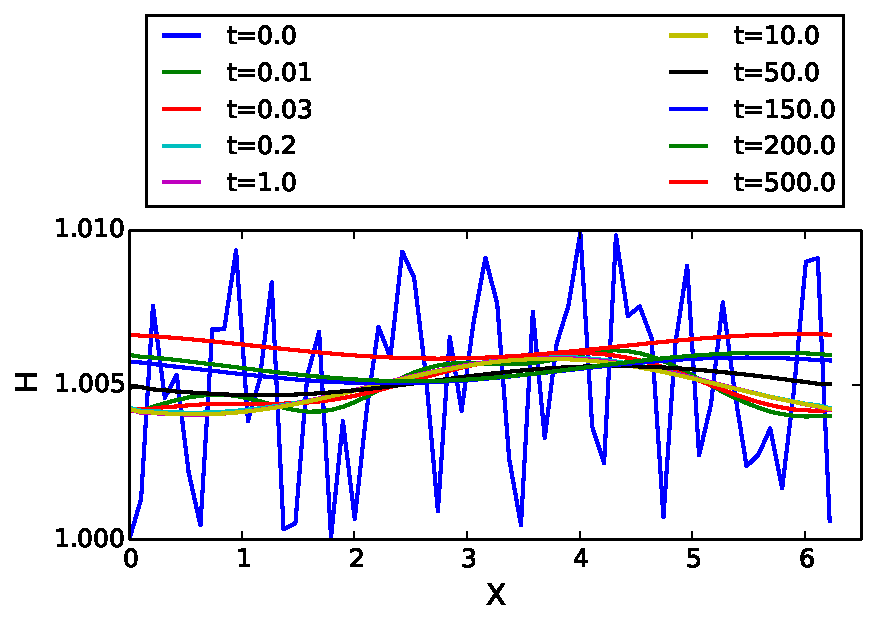
\includegraphics[]{1_98pi.pdf}
 \caption{Evolution of instability in sub-critical domain , $ L = 1.98\pi $ } \label{fig:impinge}
\end{figure}
\end{center}

\begin{center}
\begin{figure}[h!]
 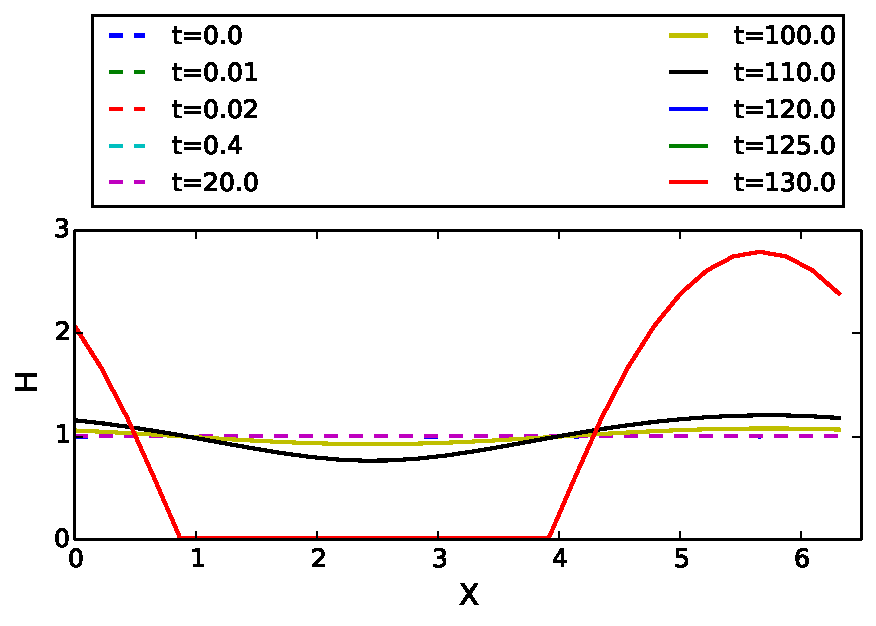
\includegraphics[]{2pi.pdf}
 \caption{Evolution of instability in slightly supercritical domain , $ L = 2.01\pi $ } \label{fig:impinge}
\end{figure}
\end{center}

\begin{center}
  \begin{figure}[h!]
 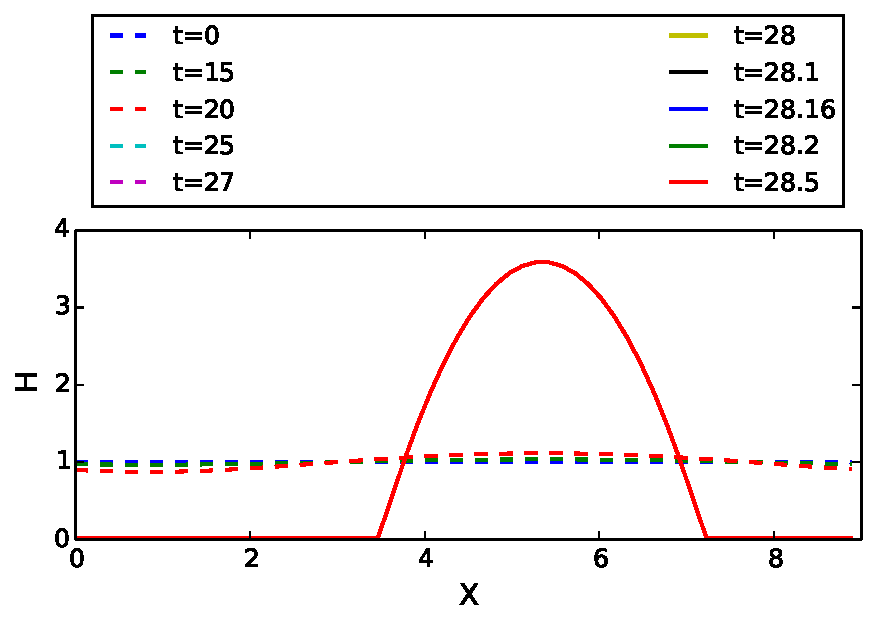
\includegraphics[]{2_2pi.pdf}
 \caption{Evolution of instability in dominant mode  , $ L = 2 \sqrt{2} \pi $ } \label{fig:impinge}
\end{figure}
\end{center}


The fig 3 depicts the evolution of instability in a sub-critical domain, L = $ 1.98 \pi $.The initial perturbations die done eventually and the instability dies down.In contrast fig 4 shows various stages of instability and film breakup and hole growth in a slightly super-critical domain of L = $ 2.01 \pi $.Note that the same initial perturbations were given in both the cases.The fig 5 gives the evolution of thin film for dominant (fastest growing) mode of linear analysis, L = $ 2 \sqrt{2} \pi $. These results are used for validation of our numerical simulation of thin films.~\cite{12}


\subsection{Current Work}

We are  parallelizing the existing Thin film code using Message Passing Interface technique with CVODE solver ~\cite{14} which have a  parallelized VODE solver.After the validation of this code we plan to couple the Thin film Model to our inhouse  conventional Navier Stokes solver which uses interface capturing technique of Volume of Fluid.  







\clearpage
\bibliographystyle{abbrv}
\bibliography{References}


\end{document}
